\section{暗物质晕的结构}

暗物质晕内部的密度并不是均匀的。我们可以用一些解析的模型来描述。

\subsection{power-law density profile}

最简单的是 幂律谱模型 (power-law density profile)

\begin{equation}
    \rho(r)=\rho_{0}\left(\frac{r}{r_{0}}\right)^{-\gamma}
\end{equation}
% $$
% \rho(r)=\rho_{0}\left(\frac{r}{r_{0}}\right)^{-\gamma}, \text { with } \gamma=\frac{9 \epsilon}{1+3 \epsilon}
% $$
在半径$r$内的质量
\begin{equation}
    M(<r)=4 \pi \int_{0}^{r} \rho\left(r^{\prime}\right){r^{\prime}}^{2} d r^{\prime}=\frac{4 \pi \rho_{0} r_{0}^{\gamma}}{3-\gamma} r^{3-\gamma}
\end{equation}

当 $\gamma \leq 3$ 时, $\lim _{r \rightarrow \infty} M(<r)=\infty$ ,总质量发散。

当 $\gamma \geq 3$ 时, $\lim_{r \rightarrow 0} M(>r)=\infty$ ,质量在暗物质晕中心发散。 

可见一个幂律谱无法描述暗物质晕的结构,需要 两个幂律谱拼起来,即 double power-law profile.


\subsection{double power-law profile}
我们希望
\begin{equation}
    \begin{cases}\rho \propto r^{-\gamma} & r \ll r_{0} \\ \rho \propto r^{-\beta} & r \gg r_{0}\end{cases}
\end{equation}
数学上给出下式满足条件
\begin{equation} \label{eq:double-pl}
    \rho(r)=\frac{\rho_{0}}{\left(r / r_{0}\right)^{\gamma}\left[1+\left(r / r_{0}\right)^{\alpha}\right]^{(\beta-\gamma) / \alpha}}
\end{equation}
% $\rho(r)=\frac{\rho_{0}}{\left(r / r_{0}\right)^{\gamma}\left[1+\left(r / r_{0}\right)^{\alpha}\right]^{(\beta-\gamma) / \alpha}} \Rightarrow \begin{cases}\rho \propto r^{-\gamma} & r \ll r_{0} \\ \rho \propto r^{-\beta} & r \gg r_{0}\end{cases}$
可以验证
当 $r \ll r_0$ 时,$1+(r/r_0)^{\alpha} \simeq 1$, \refeq{eq:double-pl} 近似为 $\rho = \rho_0 \left(\frac{r}{r_0}\right) ^{-\gamma}$. 
当 $r \gg r_0$ 时,$1+(r/r_0)^{\alpha} \simeq (r/r_0)^{\alpha}$, \refeq{eq:double-pl} 近似为 $\rho = \rho_0 \left(\frac{r}{r_0}\right) ^{-\beta}$.
为了避免 总质量发散或者中心质量发散,
要求
$\gamma < 3$, $\beta > 3$.

\subsection{NFW profile}

我们有了 double power-law profile ,但还不知道 $\alpha, \beta, \gamma$ 三个参数的取值。

N体模拟给出的 NFW profile (由 Navarro, Frenk \& White 发现) 是目前比较常用的一个好的近似模型。
% 它是一个 double power-law 模型, 
NFW profile 取 $\alpha =1$, $\beta=3$, $\gamma =1$,  其表达式为
\begin{equation} \label{eq:NFW}
    \rho(r)=\rho_{\text {crit }} \frac{\delta_{\text {char }}}{\left(r / r_{s}\right)\left(1+r / r_{s}\right)^{2}}
\end{equation}

如 \reffig{fig:NFW}  所示。
\begin{figure}[!hbtp]
	\centering 
	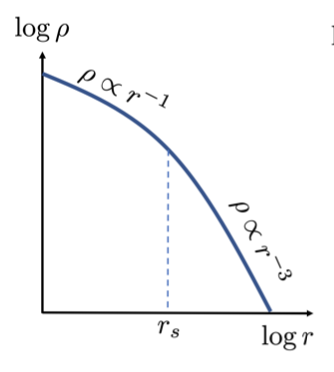
\includegraphics[width=1.0\linewidth]{NFW.png}
	\caption{NFW profile 示意图}
    \label{fig:NFW}
\end{figure}

NFW profile 存在一个问题 : Cusp-Core controversy. 
NFW profile 给出在靠近暗物质晕中心的区域, $\rho \propto r^{-1}$, 有一个高密度的“尖”,即 cusp.
但观测更倾向于 暗物质晕在中心区域密度不变, 即 “核”的结构 (core), $\rho \propto r^0$.
这对 冷暗物质理论提出了挑战。有人认为这说明 冷暗物质模型不对,他们提出了一些候选理论,比如温暗物质(warm dark matter),温暗物质是运动速度比冷暗物质快的一类粒子,这样它就会在暗物质晕形成时将中心密度较大区域的密度差异抹平。另一些人认为观测的是重子物质的分布,有可能重子物质分布和暗物质分布并不相同,重子物质在中心的分布是Core,而暗物质的分布是Cusp.
% ,用来推断
